\section{Problem Statement}
In order to develop bathymetric prediction models we must first decide which types of features will be used to predict results. 
For the scope of this project, the choice was made to compute derive statistical values from existing bathymetry grids. 
In a bathymetry grid, which is gridded bathymetry values, a single grid value represents the elevation of a physical location on Earth. 
Imagine a grid where each row represents a latitude value and each column represents a longitude value. 
This would produce a grid with 64,800 entries (360 x 180). 
Now if we have to compute a statistical value for each grid cell we would need to perform 64,800 computations. 
Since statistical computations such as mean and standard deviation require evaluating a series of data values, we have to look at each grid cells’ neighbors out to some radii. 
Therefore, in this example, we have to process 64,800 “mini” grids to get the desired results. 
To complicate things further, a one degree by one degree cell represents several square miles of Earth. 
Assigning a single elevation value to such a large space is not practical in that it does not give a true representation of the physical topology of the Earth. 
Higher resolution data sets will be required for a more accurate depiction.
The drawback is the more accurate the depiction, the larger the data set required to store the information. 
The table below shows existing bathymetry products currently available and the amount of cells and storage needed to represent the grid in memory.

\begin{figure}[h]
    \centering
    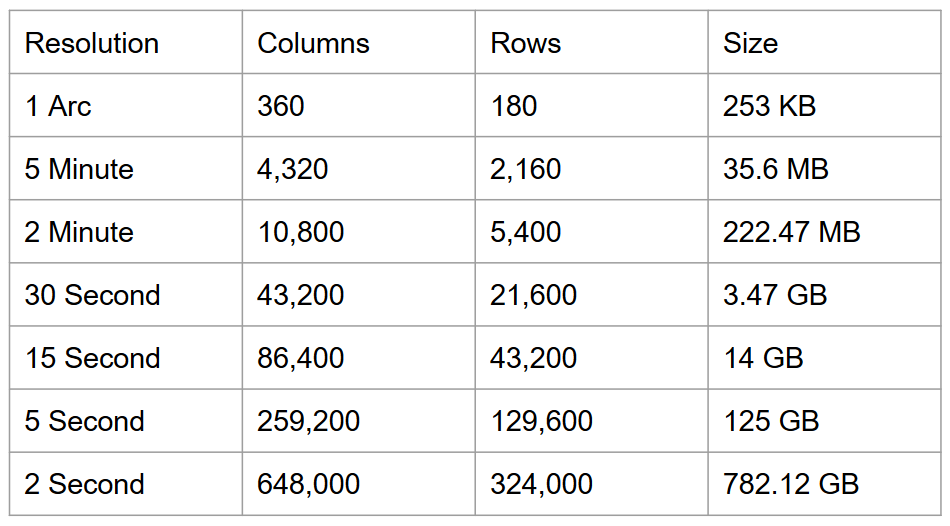
\includegraphics[scale=0.5]{grid_sizes}
    \caption{Graphic showing the sizes of grid files}
    \label{fig2:Figure 2}
\end{figure}

\par
Based on the information in Figure 2 you can see how the number of computations required to compute statistical data can grow as the resolution of the underlying bathymetry product gets larger.
In addition to the data size, the types of inputs needed to obtain optimal results is unknown. 
Based on prior work, our geophysicists will make assumptions and estimates on which types of input values may potentially produce acceptable results. 
These assumptions will be used to generate a series of input values used in model training and evaluation. 
If acceptable results are not produced, new assumptions are made and additional datasets will need to be created. 
This iterative process could occur several times over the course of this study; therefore, it is imperative for the input data generation process to be efficient.

\par
The purpose of our class project is to design a series of programs that will use varying types of parallelization to compute statistical derived data sets for use in bathymetric prediction model training. 
These data sets will be computed from high resolution existing bathymetry data sets based on guidance from the geophysicists preforming this effort. 
The goal is to find optimal implementations for performing grid based computation that produce sufficent prediction model features.
This resulting feature space will then be tested so that meaningful results may be obtained.
